%!TEX root = ../Thesis.tex
\lstset {language=C++}
% Define block styles
\tikzstyle{decision} = [diamond, draw, fill=blue!20, 
    text width=4.5em, text badly centered, node distance=3cm, inner sep=0pt]
\tikzstyle{block} = [rectangle, draw, fill=blue!20, 
    text width=5em, text centered, rounded corners, minimum height=4em]
\tikzstyle{line} = [draw, -latex']
\tikzstyle{cloud} = [draw, ellipse,fill=red!20, node distance=3cm,
    minimum height=2em]

\chapter{Blueprints en C++}
\lhead{\emph{Blueprints en C++}}

In dit hoofdstuk word gameplay logica in drie aspecten verdeeld en word voor elk aspect naar de voor en nadelen van C++ en Blueprints gekeken.

Aan de hand van deze vergelijkingen word een workflow gekozen voor het programmeren van deze logica waarin wij het beste uit C++ en Blueprints proberen te combineren.

\section{Gameplay}

Om de scheiding tussen c++ en Blueprints concreet te maken verdelen wij gameplay logica in de volgende vragen:

\begin{itemize}
	\item Wanneer moet iets gebeuren
	\item Wat moet er gebeuren
	\item Hoe moet dit gebeuren
\end{itemize}

Door deze scheiding wordt het makkelijker om de keuze tussen een C++ en een Blueprint implementatie te maken en kunnen er een aantal richtlijnen opgezet worden.

\subsection{Wanneer}
De wanneer vragen zijn vaak makkelijk te beantwoorden, bijvoorbeeld als de speler geraakt word door een projectiel wil ik dat geluid x afgespeeld word, maar moeilijk te coderen door hun asynchrone natuur. Een van de krachtigste voordelen van \gls{vs} is dat de flow van een programma uitgedrukt kan worden door middel van de lijnen tussen nodes. 

Om het verschil tussen asynchrone logica in C++ en blueprints duidelijk te maken implementeren wij hieronder het afspelen van een geluid nadat een speler dood gaat.

\subsubsection{C++}
We registeren eerst een functie die aangesproken kan worden door de timeout en het geluid wat afgespeeld word in de header van de character.

\begin{lstlisting}[caption=Registratie van de timeout functie en het geluid]	
/** Plays a sound x seconds after the death of the player*/
void AfterDeathSoundTimeOut();

/** Sound to play each time we fire */
UPROPERTY(EditAnywhere, BlueprintReadWrite, Category=Gameplay)
class USoundBase* DeathSound;
\end{lstlisting}

Vervolgens word deze functie geïmplementeerd in de character.cpp

\begin{lstlisting}[caption=Registratie van de timeout functie en het geluid]
void Adpi_unreal_colosseumCharacter::AfterDeathSoundTimeOut() 
{
	UGameplayStatics::PlaySoundAtLocation(this, FireSound, GetActorLocation());
}
\end{lstlisting}

En word de timeout voor het geluid gezet tijdens het doodgaan van de speler.

\begin{lstlisting}[caption=Implementatie van de OnDeath functie]
void Adpi_unreal_colosseumCharacter::OnDeath(const FDeathReason Reason)
{
	// death logic
	...

	FTimerHandle UnusedHandler= FTimerHandle();
	GetWorld()->GetTimerManager().SetTimer(
		UnusedHandler, 
		this, 
		&Adpi_unreal_colosseumCharacter::AfterDeathSoundTimeOut, 
		1.0f
	);
}
\end{lstlisting}

We zien hier dat de gerelateerde code op drie verschillende plekken komt te staan, tussen niet relevante code in. Pas na het lezen van de code op deze drie plekken word het duidelijk wat de complete functionaliteit is. Er zijn hier natuurlijk hulpmiddel voor zoals opmerkingen boven code te plaatsen maar bij elke extra taak die, asynchroon, uitgevoerd moet worden word de code complexer en moeilijker te begrijpen. De lezer moet namelijk alle gerelateerde functionaliteit in zijn geheugen hebben.

\subsubsection{Blueprints}
In Blueprints zou deze logica er als volgt uit zien:

\begin{figure}[!ht]
  \centering
    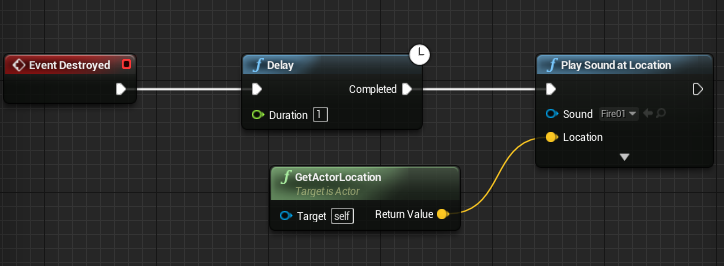
\includegraphics[width=\linewidth,height=\textheight,keepaspectratio]{OnDestroyedSoundDelay}
    \caption{Afspelen van een geluid na het doodgaan van de speler in Blueprints.}
\end{figure}

In de blueprint implementatie is het in een oog opslag duidelijk dat er een geluid afgespeeld word op de locatie van de speler een seconde nadat deze deze dood gaat. De logica bevind zich op de dezelfde plek en de witte lijnen geven de flow van de logica aan. 

Een ander groot verschil dat we hier zien is dat er voor iets simpels als een vertraging in tekstuele code naast de standaard kennis van de c++ syntax ook kennis nodig is van de volgende concepten:

\begin{itemize}
	\item Pointers
	\item Pass by reference
	\item Function references
	\item Namespaces
	\item Out parameters (de UnusedHandler)
	\item Floats
	\item Types
	\item Macros. 
\end{itemize}

Terwijl in Blueprints all deze concepten verborgen zijn in de nodes. Het verbergen van de onderliggende werking van functionaliteit is een thema wat vaker terugkomt in programmeren en wordt aangemoedigd. Het verbergen van deze logica heeft als gevolg dat er zonder programmeer kennis de wanneer logica geïmplementeerd kan worden.

\subsection{Wat}

Het plaatsen van de wat logica in Blueprints of c++ is lastiger om te bepalen. Voor logica die de niet-programmeurs schrijven is c++ geen optie en moet dit wel in Blueprints maar voor programmeurs moet er een afweging gemaakt worden.

Het probleem ontstaat voornamelijk bij complexe conditionele logica.

\subsubsection{Conditionele Logica}

Als we de conditionele logica van het afvuren van de events van een.
LookEventsComponent[zie hoofstuk ?] in c++ en blueprints met elkaar vergelijken.

\begin{itemize}
	\item Bijlage 1: Tick functie van de LookEventsComponent \ref{appendix:LookEventsLogicC}
	\item Bijlage 2: Conditional logic van Tick functie van LookEvents in Blueprints \ref{appendix:LookEventsLogicBlueprints}
\end{itemize}

Zijn beide varianten moeilijk te lezen. Voor iemand die niet codeert ziet de Blueprints variant er waarschijnlijk begrijpgaarder uit maar de complexiteit komt voornamelijk door de logica zelf en in tekstuele code zijn er een aantal manieren om dit soort constructies kleiner te maken zoals:

\begin{lstlisting}[caption=Early return in een complexere if statement in c++]
if (bActive != true || (bShouldUsedOnce && TimesUsed > 0) || bIsInTimeOut == true) 
{
	return;
}
\end{lstlisting}
In vergelijking met 

\begin{figure}[!ht]
  \centering
    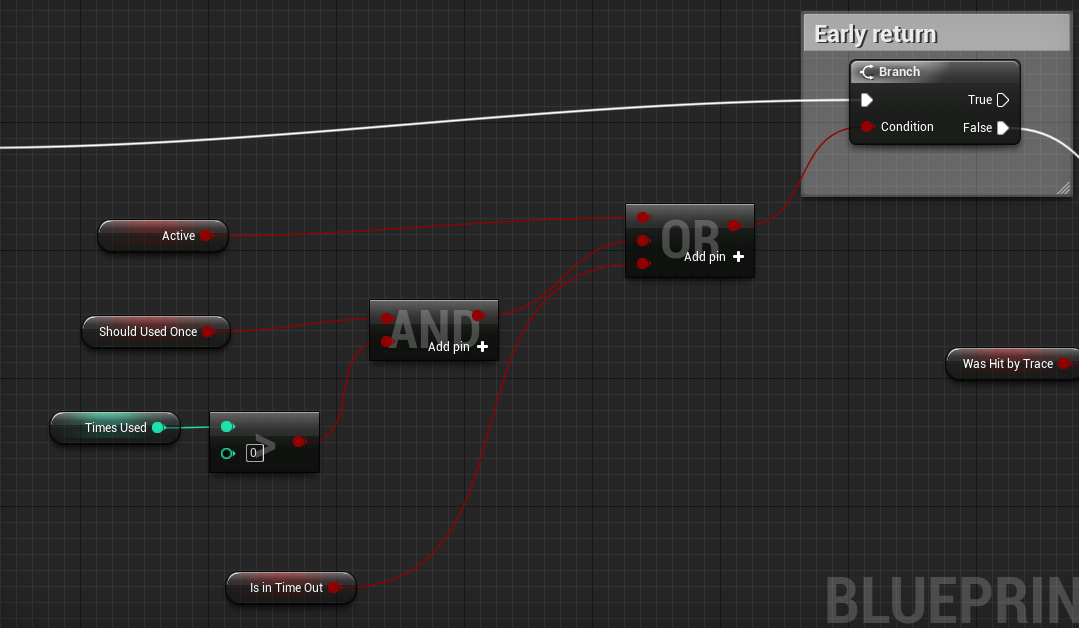
\includegraphics[width=\linewidth,height=\textheight,keepaspectratio]{EarlyReturnBluePrint}
    \caption{Early return in een complexere if statement in Blueprints.}
\end{figure}

Een ander voorbeeld is de volgende functie die bepaald of de trigger van een LookEventsComponent onderdeel was van een trace.

\begin{lstlisting}[caption=Een functie die kijkt of de huidige component geraakt is door een trace]
FHitResult ULookEventsComponent::WasHitByTrace(const TArray<FHitResult> HitResults) 
{
	UObject* Trigger = (bIsBeingWatched) ? UnSeenTrigger : SeenTrigger;

	for (auto& HitResult : HitResults)
	{
		UObject* HitObject = (Trigger->IsA(AActor::StaticClass())) ? Cast<UObject>(HitResult.GetActor()) : Cast<UObject>(HitResult.GetComponent());	

		if (HitObject == Trigger)
		{
			if (bShouldDrawTriggerDebug) {
				DebugTrigger(HitObject, 0.1f);
			}
			return HitResult;
		}
	}
	return FHitResult();
}
\end{lstlisting}

In vergelijking met:

\begin{figure}[!ht]
  \centering
    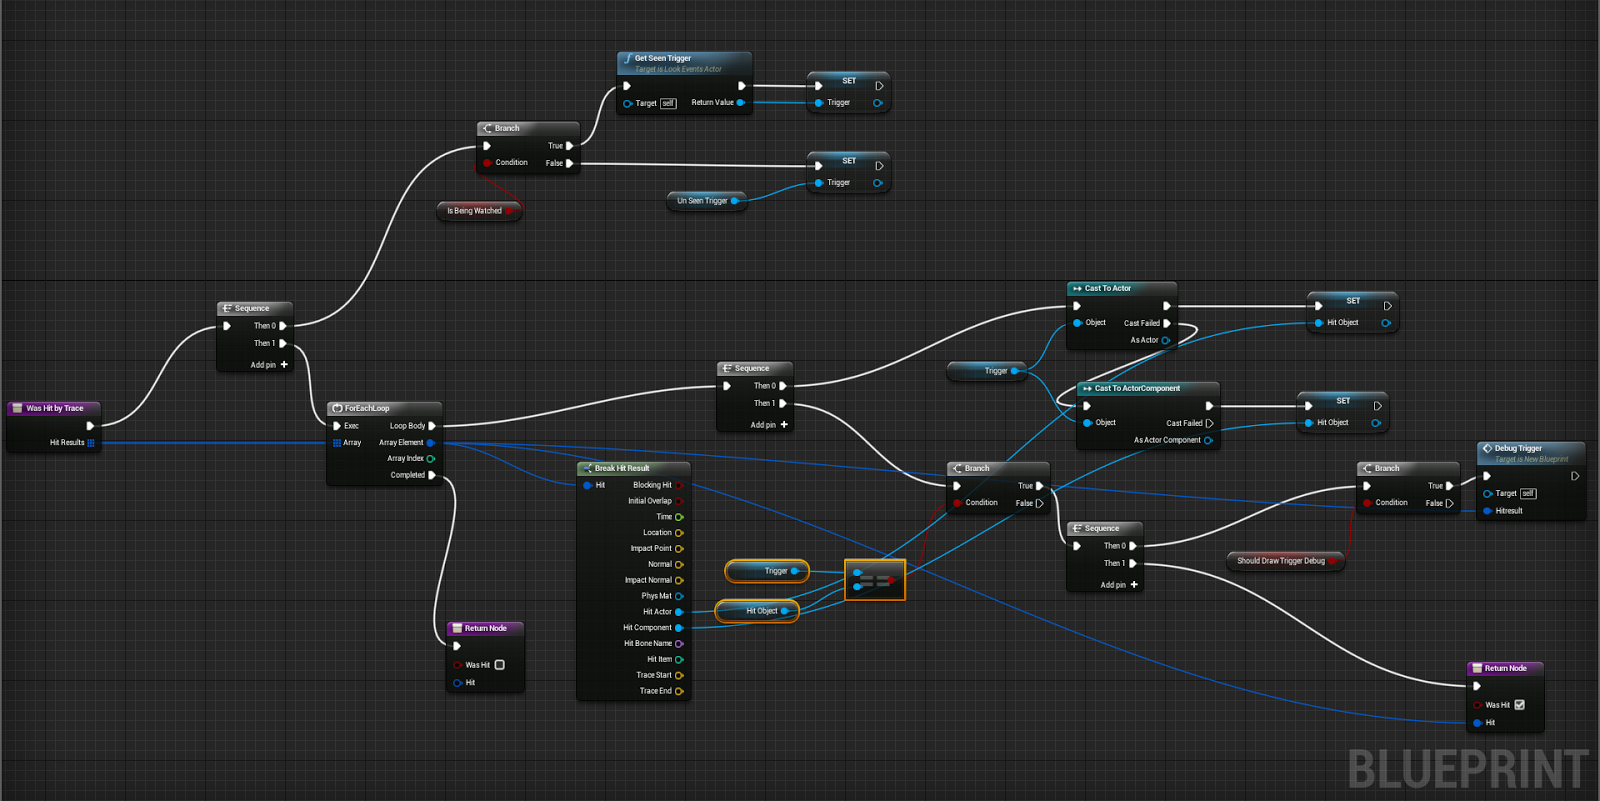
\includegraphics[width=\linewidth,height=\textheight,keepaspectratio]{WasHitBytTraceBluePrintExample}
    \caption{Een Blueprint die kijkt of de huidige component geraakt is door een trace.}
\end{figure}

Voor complexe conditionele logica is c++ sneller te begrijpen en geeft meer mogelijkheden om dit te versimpelen. 

\subsection{Hoe}
Met de hoe vraag word de interne werking van een functionaliteit bedoelt waaronder ook de integratie met de rest van het programma, denk aan integratie met de rest van de engine, lifecycles, overerving en performance.

Complexe algoritmes zijn altijd makkelijker in C++ voor zowel leesbaarheid als onderhoudbaarheid. Daarnaast is de scheiding van algoritmes met de rest van de code belangrijk voor het scheiden van complexiteit.

\subsection{Onderhoud en Performance}
Naast het schrijven van de logica zijn performance en onderhoud twee onderwerpen die door elk aspect van een spel verwikkeld zijn en daarom ook onderdeel moeten zijn voor onze keuze van workflow.

\subsubsection{Onderhoud}
Naast een kleine verbetering in leesbaarheid heeft het schrijven van logica in c++ een ander belangrijke voordelen. Namelijk de voordelen van een code editor. Dit geeft uitgebreide debug, zoek en meta informatie. 

De error’s die de \gls{ue4} voor je genereed zijn niet altijd even duidelijk, voornamelijk error’s die pas tijdens het packagen van een project ontstaan, en het vinden van een foutieve Blueprint kan extreem lastig zijn. Bijna elk element in de \gls{ue4} kan Blueprints code bevatten. En elk element op zich kan die Blueprints weer in kleinere elementen verdelen. Deze elementen bevinden zich tussen alle andere soorten assets zoals Meshes, Animaties, Deciscion Trees, Materials, Textures etc en het zoeken van een onbekende fout hierin is extreem lastig.

Als de foutieve code in c++ had gestaan kan er altijd door middel van een stack trace gekeken worden in welke functie het fout gaat en kan er gezien worden welke functie die functie aansprak en verder omhoog. 

Het auto aan vullen van functie namen en informatie tonen over functies door middel van de JavaDoc opmerking notatie versimpelt het schrijven van complexe code die gebruikt maakt van de \gls{ue4}. 

\subsubsection{Performance}
Een ander belangrijk onderdeel van de hoe logica is performance. De performance van Blueprints is namelijk lager dan dat van c++. In de hoe en wat vraag is dit verschil compleet onmerkbaar maar in code wat vaak, bijvoorbeeld in de loop van een game, word uitgevoerd kan het verschil merkbaar worden.
In c++ is er ook veel meer controle over de manier waarop de computer logica interpreteert, in Blueprints is dit een stuk minder duidelijk. Dit zorgt ervoor dat op een lager niveau optimalisaties mogelijk zijn. 

Daarnaast is het makkelijker om complexe optimalisaties te schrijven op een onderhoudbaar manier. Als er bijvoorbeeld een performance probleem ontstaat in het aantal raytraces wat de LookEventsComponents nodig hebben is het mogelijk om een cache te schrijven voor de ray traces waar de LookEventsComponent een trace uit vraagt als deze trace dan al eerder door een andere LookEventsComponent berekend is krijg hij de resultaten van die trace inplaats van een nieuwe trace te maken.

\subsection{Conclusie}
Voor de wanneer vraag is Blueprints voor zowel de programmeur als de niet-programmeur altijd de beste optie. Niet alleen is het leesbaarder maar ook flexibeler doordat de logica op een logische manier achter elkaar staat.

Voor de hoe vraag is C++ altijd de beste optie. Onderhoudbaarheid en performance spelen hier een belangrijke rol. 

Voor de wat vraag heeft de niet-programmeur geen optie maar de programmeur wel. Voor triviale code kan er gekozen worden voor Blueprints maar voor complexe conditionele logica heeft C++ de voorkeur. 

\section{Workflow}
Voor onze workflow willen wij de complexiteit voor de niet-programmeurs zo laag mogelijk houden met zo veel mogelijk vrijheid. Daarnaast is flexibiliteit belangrijk voor het makkelijk en veilig experimenteren en itereren.

Gebaseerd op het verdelen van de gameplay logica in de drie vragen hoe, wat en wanneer word er voor de volgende workflow gekozen.
    
\begin{figure}[H]
	\centering
		\begin{tikzpicture}
			[node distance=.8cm,
			start chain=going below,]
				\node[punktchain, join] (Experimenteren) 	
					{Experimenteren (Blueprints)};
				\node[punktchain, join] (hoe)      			
					{Implementatie hoe (C++)};
				\node[punktchain, join] (wat)    			
					{Implementatie complexe wat (C++)};
				\node[punktchain, join] (overerving) 		
					{Blueprints overerving (Blueprints)};
				\node[punktchain, join] (wanneer) 			
					{Wanner en wat (Blueprints)};
		\end{tikzpicture}
		\caption{Workflow voor het programmeren voor de Unreal Engine 4.}
\end{figure}

Elk component zal beginnen als een imperfecte Blueprint logica. In dit stadium is de performance en onderhoud niet belangrijk, en hoeft het niet eens compleet functioneel te zijn. Er kan direct ge-experimenteert en getest worden. Dit kan niet alleen waardevolle informatie opleveren voor het design aspect van een project maar plaats de logica ook in de context van het project. Vaak komt hier gewenste functionaliteit uit die tijdens het bedenken over het hoofd gekeken is.

Nadat het duidelijk is dat het component gebruikt gaat worden in het project en de gewenste functionaliteiten duidelijk zijn kan er een fatsoenlijke en efficiënte C++ implementatie geschreven worden.

De C++ implementatie word vervolgens overerft door een Blueprint die de aanvullende logica toevoegt.

Ook in gevallen waarin de Blueprint niet iets toe te voegen heeft is het belangrijk om toch een Blueprint te maken van de C++ code. Er kan hierdoor namelijk makkelijk mee geëxperimenteerd worden en niet-programmeurs hebben hierdoor ook de mogelijkheid om iets toe te voegen of een standaard waarde te veranderen.

\section{Versie Controle}
Versie controle is een belangrijk onderdeel van elk ICT project en al valt dit buiten de scope van deze scriptie word er hier een korte vermelding van gemaakt.

Versie controle is een belangrijk onderdeel in samen werken aan code en speelt een belangrijke rol in het onderhoud van code. Er zijn tools in \gls{ue4} om versie controle tools zoals git en svn op Blueprints, en assets, toe te passen. Voor deze scriptie is de plugin ontwikkeld met behulp van git maar is er niet gekeken naar een manier waarop niet-programmeurs hier ook mee kunnen werken.

Tijdens de interviews[?] werd het duidelijk dat er geen bestaande kennis van versie controle aanwezig was in de visuele teams van DPI. Het kiezen, opzetten en leren van versie controle en de integratie hiervan met de \gls{ue4} valt buiten de scope van deze scriptie.